\chapter{Introdução}

Escrever um trabalho científico pode ser uma tarefa desafiadora. \cite{severino}
destaca a complexidade e o rigor necessários na elaboração de trabalhos científicos, que não
apenas envolvem o domínio do conteúdo específico, mas também a aderência às normas
técnicas para apresentação formal e formatação correta.

A Associação Brasileira de Normas Técnicas 
(\acrshort{abnt})
, é a entidade responsável por,
dentre outras, fornecer as normas que regulam o processo de criação de trabalhos acadêmicos.
A Norma Brasileira Regulamentadora 
(\acrshort{nbr})
 Nº 14724, por exemplo: Especifica os princípios
gerais para a elaboração de (teses, dissertações e outros), visando sua apresentação à
instituição (banca, comissão examinadora de professores, especialistas designados e/ou
outros)
\cite{abnt}.

Ademais, ainda com respeito aos trabalhos acadêmicos, não somente a
regulamentação da 
\acrshort{nbr}
14724 deve ser observada. Há ainda a 
\acrshort{nbr}
6023 que trata a respeito
da elaboração de referências e a 
\acrshort{nbr}
10520, que diz respeito às citações em documentos.

\cite{castro}, adverte que: "Em ciência, não pode haver uma
separação entre forma e conteúdo. Trata-se de uma separação fictícia, pois fica se conhecendo
o conteúdo pela forma." Ou seja: A forma do trabalho, sua apresentação, sua formatação e
todo o seu arranjo gráfico é tão importante quanto seu conteúdo. 
\cite{medeiros} vai
complementar essa visão, afirmando que a apresentação gráfica "[...] contribui para a
consecução de um trabalho capaz de atingir seu objetivo. Monografia realizada sem a
preocupação gráfica, em geral, acaba malsucedida."

Em seu artigo, 
\cite{SilvaVitoria}
vão analisar as percepções e dificuldades dos
alunos de um curso superior em Tecnologia de Gestão em Recursos Humanos. Dentre suas
dificuldades, (dos alunos em questão), é destacada a questão da formatação do trabalho
acadêmico. Há também o fato de que as bancas avaliam os trabalhos baseadas em critérios da
própria Instituição de Ensino Superior (
\acrshort{ies}
), critérios estes que não estão necessariamente
presentes nas normas da \acrshort{abnt}, ou seja, há uma subjetividade presente que não é comum a
todas às \acrshort{ies} quanto a questão da formatação. Essa subjetividade contribui para a confusão dos
alunos, pois a \acrshort{ies} avaliará de acordo com aquilo que julga apropriado, o que muitas vezes
pode obscurecer o direcionamento do aluno ao redigir/formatar seu trabalho."

\clearpage

\cite{santos}
em seu Trabalho de Conclusão de Curso
(\acrshort{tcc})
, também analisa as
dificuldades encontradas por egressos, desta vez do curso de Ciências Contábeis da
Universidade Federal da Paraíba
(\acrshort{ufpb}).
Em sua pesquisa é destacado que "Quanto a
formatação do trabalho com as normas da 
\acrshort{abnt}, [...], 60\% teve alguma dificuldade, inclusive
32\% teve muita dificuldade.", ou seja, a formatação do trabalho é um grande desafio presente
na vida de boa parte dos estudantes em processo de escrita.

\section{Objetivo}

Levando em consideração os problemas que os alunos de diversas instituições de ensino enfrentam ao elaborar seus respectivos
trabalhos (conforme apresentado acima), o objetivo deste instrumento é desenvolver uma plataforma web de alta
interatividade\footnote{Refere-se à capacidade de um sistema, aplicação ou interface de responder
        às ações do usuário de maneira eficaz e intuitiva}
e
inteligibilidade\footnote{Refere-se à clareza e compreensibilidade da interface, documentação e feedback fornecidos pelo
    sistema. Um software inteligível facilita o entendimento do usuário sobre como utilizá-lo e quais são os resultados de suas ações.},
de modo que o discente possa se preocupar apenas com o conteúdo. Os detalhes de formatação, de acordo com os padrões da
\acrshort{abnt}
e da
\acrshort{ies},
ficarão a cargo da própria plataforma.

A criação de um trabalho de
\acrshort{tcc}
se dará basicamente por três passos básicos: Escrita em blocos;
\textit{Parsing}\footnote{O termo Parsing, (do inglês: análise), será utilizado no
sentido de analisar e transformar algo em outra coisa.}
e
Documento em
\acrshort{pdf}
. A Figura\ref{fig:Passos para criar um documento} ilustra esse fluxo na linha do tempo.

\begin{figure}[ht]
    \centering
    \caption{Passo a passo para criar um documento na plataforma}
    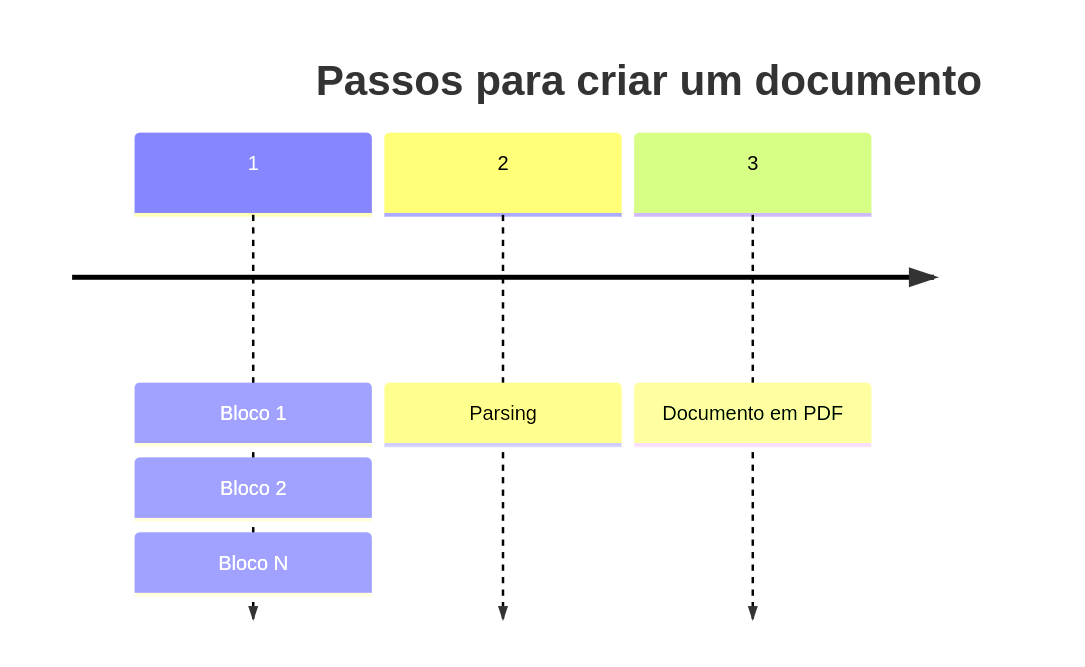
\includegraphics[width=0.8\textwidth]{./images/Passos para criar um documento.png}
    \label{fig:Passos para criar um documento} \\
    \textnormal{\fontsize{10pt}{12pt}Fonte: Autoria própria}
\end{figure}

O usuário interagirá com a aplicação escrevendo blocos que serão transformados
no documento final em
\acrshort{pdf}
. A este processo daremos o nome de Parsing. Após este, bastará
enviar o download do \acrshort{pdf}
ao usuário com todo o padrão de formatação. Os trabalhos desenvolvidos nesta plataforma
terão então duas versões: A versão de blocos, (sem formatação e interativa); e a versão
final já formatada em \acrshort{pdf}.

\section{Fluxo do documento}

\subsection{Escrita em blocos}

A escrita se dará de modo em que tudo será considerado um bloco.
A escrita em blocos consiste numa abordagem em que o texto vai sendo
escrito em seu fluxo natural, porém blocos podem ser adicionados à escrita.
Um bloco é um elemento adicionado ao fluxo de trabalho que desenpenha um papel
que o diferencia dos demais blocos.
Por exemplo: Uma imagem pode ser considerada um bloco nesta abordagem, uma vez
que não é um texto mas tem o objetivo de fornecer informações visuais. O próprio corpo
do texto em si será considerado um bloco, denominado parágrafo. Um título será um bloco
textual cujo objetivo será separar sessões do texto coesas. Uma lista será um bloco para enumerar
intens e assim por diante. O documento será basicamente uma composição de diversos blocos dispostos de forma a formar
uma unidade coesa final, que será o trabalho propiamente dito.

\subsection{Bloco}

Um bloco é uma unidade lógica no documento que desenpenha um papel especializado que nenhum
outro bloco o faz. Por exemplo: O bloco mais importante da
plataforma\footnote{O termo plataforma será utilizado
    de forma intercambiável e como sinônimo de aplicativo; sistema web; ou aplicativo da web}
será o de texto, (denominado bloco parágrafo), pois sem texto, não há trabalho.
Sem texto não há tão pouco comunicação que transmita informação
de caráter acadêmico-científico.

Semelhante ao bloco de texto, diversos outros blocos adjascentes
auxiliarão na construção do documento acadêmico. O bloco de imagem, por
exemplo, ajuda a exibir informações de forma ilustrativa e auxilia bastante
em exemplos que estão sendo dados em determinado contexto do texto.

A maior parte dos blocos contará com uma espécie de submenu, (em termos de aplicação),
que os permita personalizar. A personalização de blocos é importante para editar
configurações e dar autonomia ao usuário em determinar mais precisamente o papel
daquele bloco no texto. Por exemplo: Um bloco de título ajuda a separar o texto
em unidades coesas. Porém, existem diversos tipos de títulos: Existe o título, o
subtítulo, e até o subtítulo do subtítulo.

O submenu será a configuração que o usuário fará no bloco após escolhê-lo. No
caso do título, por exemplo: Após o usuário escolher este bloco, poderá configurar
o nível de título desejado. Nível este que varia do 1 ao 4, sendo 2; 3 e 4
espécies de subtítulos. No caso de uma imagem, o submenu funcionará para que possa
ser definida a imagem, bem como seu título de sua descrição.

A imagem abaixo ilustra a composição de um trabalho com seus respectivos blocos:

\begin{figure}[ht]
    \centering
    \caption{Divisão de blocos em uma imagem}
    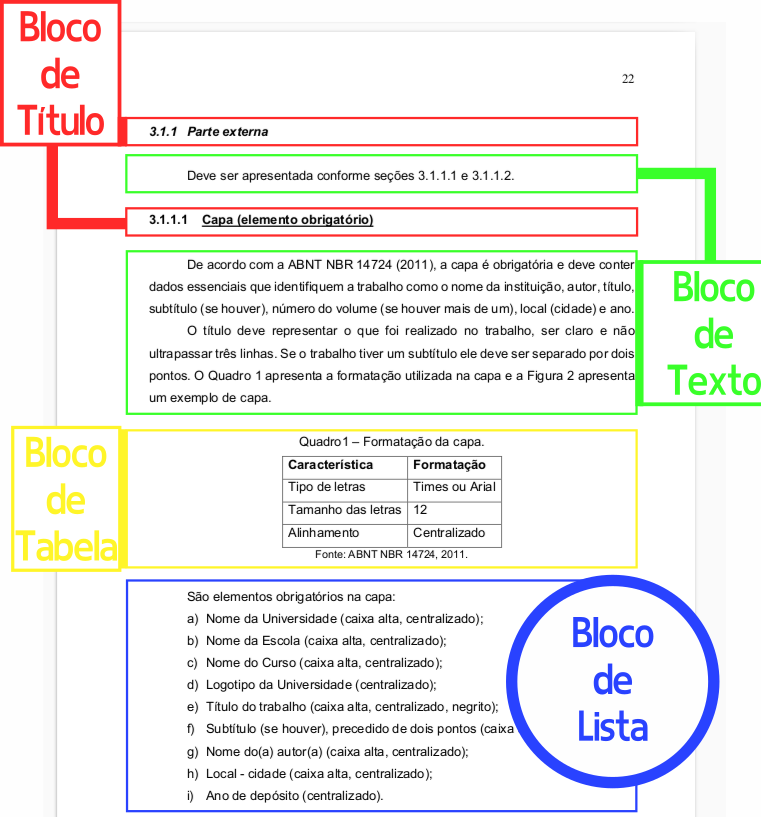
\includegraphics[width=0.8\textwidth]{./images/blocos-no-documento.png}
    \label{fig:blocos-no-documento} \\
    \textnormal{\fontsize{10pt}{12pt}Fonte: Adaptado de \cite{pucgo}}
\end{figure}

\subsection{Parsing}

O processo de Parsing é o processo que acontecerá sempre que o usuário desejar
ver o
\textit{layout}\footnote{Do inglês: Disposição, ou esboço. Esta palavra geralmente está associada ao desenho ou visual de algo.
}
da versão final de seu trabalho. Ele usa o código intermediário gerado pelos blocos para montar o
\acrshort{pdf}
final.

Este processo é, em termos simples, uma espécie de análise a ser aplicada no código gerado pelos blocos
da aplicação. A plataforma gerará um código
\acrshort{json}\footnote{Ver (sessão que trata do JSON)
}
como resultado das interações do usuário, que posteriormente
serão convertidos em código
latex\footnote{Ver (sessão que trata do latex)
}.
Só então, finalmente será utilizado um utilitário que converterá o código latex
em um documento
\acrshort{pdf}. A
Figura\ref{fig:app-json-latex-pdf} ilustra esse processo:

\begin{figure}[ht]
    \centering
    \caption{Etapas do processo de Parsing}
    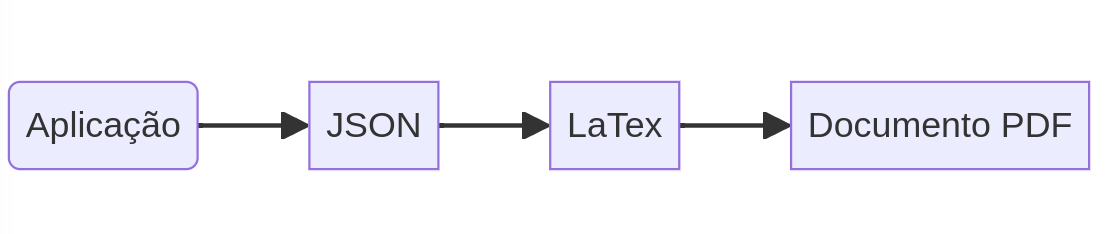
\includegraphics[width=0.9\textwidth]{./images/app-json-latex-pdf.png}
    \label{fig:app-json-latex-pdf} \\
    \textnormal{\fontsize{10pt}{12pt}Fonte: Autoria própria.}
\end{figure}

\section{Ambiente de desenvolvimento}

O ambiente de desenvolvimento é de extrema importância para que todas as ferramentas
utilizadas possam funcionar em perfeita harmonia em suas respectivas integrações e
colaborações. Muitas vezes, problemas de compatibilidade podem afetar
o funcionamento das mesmas e impedir que o programa final
seja executado corretamente, causando
\textit{bugs}\footnote{Do inglês: Inseto. Esta palavra é muito utilizada no contexto de desenvolvimento de aplicativos
para se referir a problemas que afetam o funcionamento dos mesmos
}
e outros imprevistos impeditivos tanto para a correta execução, quanto
para a exeperiência de desenvolvimento.
A lista abaixo diz respeito às ferramentas e ao ambiente onde este \textit{software}
foi desenvolvido, bem como todas as suas respectivas versões:

\clearpage

\subsection{Lista de tecnologias do ambiente de desenvolvimento}

\begin{itemize}
        
	\item Npm 10.2.3
	\item Yarn 1.22.19
	\item NodeJs 20.10.0
	\item kpathsea version 6.3.4/dev
	\item Sistema Operacional: Ubuntu 20.04
	\item makeglossaries (Utilitário latex)
	\item BibTeX 0.99d (TeX Live 2022/dev/Debian)
	\item pdfTeX 3.141592653-2.6-1.40.22 (TeX Live 2022/dev/Debian)
    
\end{itemize}

\chapter{Fundamentação teórica}

A plataforma será construída sob alguns pilares fundamentais indispensáveis
a seu funcionamento. São estes pilares que garantirão o sucesso e o correto
funcionamento da aplicação, afim de que todo o objetivo discutido até o
presente momento seja atingido.

A
Figura\ref{fig:pilares-da-plataforma}
mostra em forma de mapa mental todos os principais pilares sobre os quais
o aplicativo será contruído. Estes pilares são formados por diversas
tecnologias, bibliotecas,
\textit{frameworks}\footnote{Uma framework é como um kit de ferramentas pré-pronto que fornece uma gama
    de funcionalidades pré-construídas e testadas afim de facilitar o processo
    de desenvolvimento. \cite{amazon-framework}
}
e conceitos que deverão trabalhar de forma integrada.

\begin{figure}[ht]
    \centering
    \caption{Pilares da plataforma, (mapa mental)}
    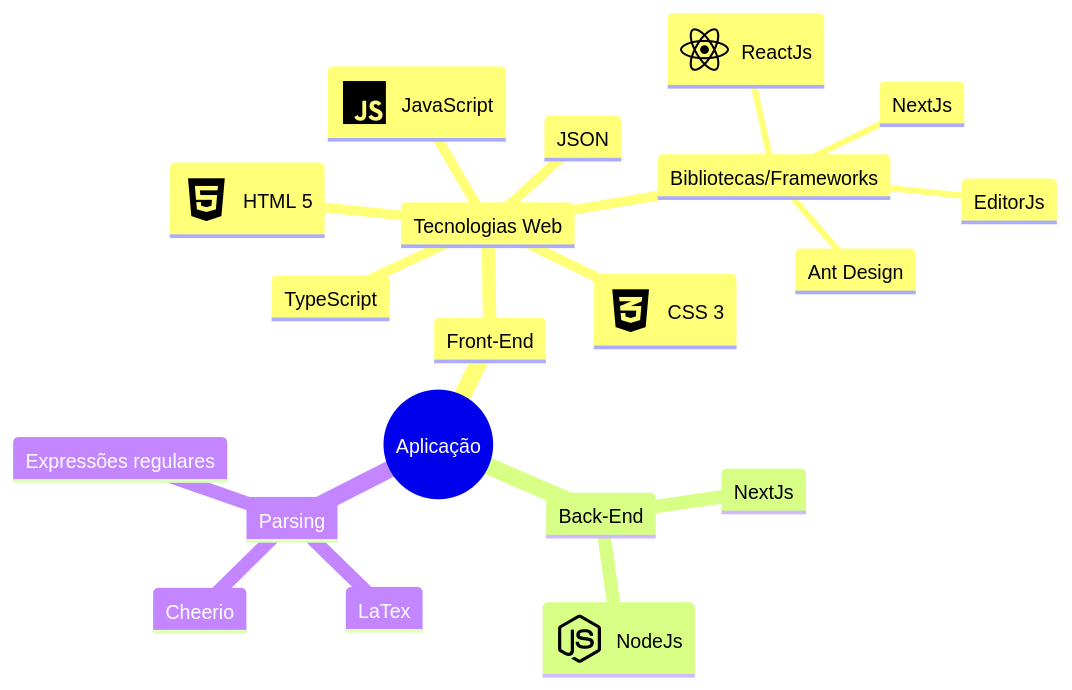
\includegraphics[width=0.9\textwidth]{./images/pilares-da-plataforma.png}
    \label{fig:pilares-da-plataforma} \\
    \textnormal{\fontsize{10pt}{12pt}Fonte: Autoria própria.}
\end{figure}

Estes pilares estão subdivididos em três grandes subcategorias, a saber: Front-End;
Back-End e Parsing. Cada qual com seus respectivos conceitos e tecnologias.

\section{Do Front-End}

O Front-End é, basicamente, a "linha de frente". É a parte da aplicação que interagirá
diretamente com o usuário. Ao profissional que codifica e desenvolve esta parte do
projeto, damos o nome de Desenvolvedor Front-End. A interface do usuário, que é
onde o mesmo realiza suas interações com o sistema, normalmente é desenhada por
um
\textit{designer}\footnote{Profissional que atua com design.
}
, ficando a cardo do desenvolvedor o papel de adaptar o
\textit{design}\footnote{Do inglês: Desenho.
}
ao código afim de obter os efeitos desejados.
\cite{totvs-front-end}

\subsection{Tecnologias web}

As tecnologias
\acrshort{web}
desempenham um papel crucial na criação de experiências
digitais interativas, permitindo que os usuários se envolvam com o conteúdo de maneira mais
dinâmica e significativa. A incorporação da
\textit{Internet}\footnote{Rede mundial de computadores, \cite{marco-civil-art-2}.
}
na vida diária resultou em mudanças
significativas, marcada por um ritmo de evolução e aprimoramento sem precedentes, além da
distribuição de conteúdo em massa. Juntamente com essas mudanças, surgiram novas
tecnologias, variando de
\textit{softwares}\footnote{O software é o conjunto de instruções dadas a um computador, de modo que
    ele execute determinada tarefa. Podemos dizer que o software é
    a parte lógica do sistema computacional.  \\   \cite{hardware-e-software}.
}
a
\textit{hardwares}\footnote{Com hardware, compreende-se o equipamento físico de um sistema computacional.
    Suas unidades Lógicas de Processamento, memórias e unidades de armazenamento são
    hardware. \\ \cite{hardware-e-software}.
},
aprimorando a experiência de navegação na
\acrshort{web}
\cite{molgado}.

A Internet, que teve origem nos Estados Unidos em 1969, foi inicialmente utilizada
por universidades, governos e instituições financeiras antes de se expandir globalmente. No
início, a internet era uma via de mão única onde os usuários consumiam informações e se
comunicavam de maneira privada. A evolução começou com a introdução de sistemas de
busca avançados, destacando-se o lançamento do Google em 1998, que democratizou o
acesso à informação.
\cite{vitoriano}.

A grande reviravolta na internet aconteceu em 1999, com o surgimento do
\textit{Blogger},
marcando o início da
Web
2.0, onde a comunicação tornou-se bidirecional. Os usuários
passaram a gerar conteúdo e se relacionar publicamente com marcas, empresas e pessoas por
meio de comentários, além de consumir informação. A evolução da tecnologia móvel, em
conjunto com o surgimento de redes sociais como
\textit{Fotolog},
\textit{MySpace},
\textit{Orkut},
\textit{Facebook},
\textit{YouTube}
e
\textit{Twitter},
ampliou o conceito de Web 2.0, permitindo o compartilhamento de fotos,
vídeos e textos em uma escala maior.
\cite{vitoriano}.

A forma como se interage com a internet também evoluiu ao longo do tempo.
Passou-se de sites estáticos para interativos e animados, chegando até aos sites totalmente
responsivos\footnote{A responsividade é a capacidade de uma página da
    \acrshort{web}
    em se adaptar a diferentes dispositivos e tamanhos de tela.
    \cite{responsivo}
}
e adaptáveis de hoje. Isso foi possível devido ao desenvolvimento de novos
gadgets e ao surgimento de novas linguagens de programação. Atualmente, a Web Moderna é
composta por várias técnicas, metodologias, linguagens e ferramentas que permitem o
desenvolvimento de aplicações conectadas e interativas, oferecendo diversas formas de
interação com interfaces digitais.
\cite{vitoriano}.

\subsubsection{Linguagem de Marcação de Hipertexto, HTML}

A Linguagem de Marcação de Hipertexto, do inglês: HyperText Markup Language
(\acrshort{html})
foi criada por Tim Berners-Lee enquanto trabalhava na Organização Europeia para a
Pesquisa Nuclear
(\acrshort{cern}),
o laboratório de física de partículas na Suíça, no final dos anos
1980 e início dos anos 1990. O objetivo era criar uma maneira de compartilhar documentos e
informações em um ambiente de rede. A primeira versão do
\acrshort{html}
tinha apenas 18 elementos
de marcação, permitindo a formatação básica de texto e a inclusão de
\textit{links}\footnote{Do inglês: Ligação. Também chamado de hiperlink, é uma referência a um
    documento eletrônico que, quando clicado, leva o usuário para outro recurso
    ou documento.
},
imagens e listas.
\cite{w3c}.

O
\acrshort{html}
rapidamente ganhou popularidade e passou por várias iterações, cada uma
adicionando novos elementos e funcionalidades. O
\acrshort{html}4,
lançado em 1997, trouxe uma
série de melhorias, incluindo mais controle sobre a aparência das páginas web, a introdução
de folhas de estilo em cascata
(\acrshort{html})
e melhor suporte a
\textit{scripts}\footnote{Do inglês: Roteiro. Aqui usado no sentido de código fonte, que nada mais são
    do que um conjunto de instruções que o computador seguirá de modo interpretativo.
}.
\cite{w3c}.

Finalmente, o
\acrshort{html}5,
lançado oficialmente em 2014 pelo World Wide Web
Consortium (\acrshort{w3c}), trouxe uma série de novas funcionalidades, incluindo suporte nativo para
vídeo e áudio; novos elementos semânticos; gráficos e animações; geolocalização;
armazenamento local e muito mais.
\cite{w3c}.

\subsubsection{Funcionamento do HTML}

O
\acrshort{html}
funciona como uma linguagem de marcação, o que significa que ele usa
\textit{"tags"}\footnote{Do inglês: Marcação.
}
para definir diferentes partes de um documento. Essas tags informam ao navegador
como exibir o conteúdo da página. Por exemplo, a tag
<p>
é usada para definir um parágrafo,
enquanto a tag
<h1>
é usada para definir um cabeçalho de primeiro nível.
\cite{w3c}.

As páginas
\acrshort{html}
são estruturadas usando uma combinação de elementos de bloco,
(que formam a estrutura principal da página), e elementos
\textit{inline}\footnote{Do inglês: Dentro da Linha. São elementos que podem ser escritos sem quebra de linha.
},
(que formatam o conteúdo
dentro desses blocos). Os elementos são aninhados dentro de outros elementos para criar a
estrutura hierárquica da página.
\cite{w3c}.

\subsubsection{HTML versão 5}

Com o
\acrshort{html}5,
os desenvolvedores podem criar jogos online, reproduzir vídeos e
áudios diretamente no navegador, tudo isso sem a necessidade de instalação de plugins
externos. Isso resultou em uma melhor experiência geral do usuário, com carregamento mais
rápido e maior compatibilidade entre os navegadores.
\cite{w3c}.

Além disso, o
\acrshort{html}5
também trouxe recursos avançados de armazenamento local,
como o
\textit{\acrshort{web} Storage}\footnote{O termo
    \acrshort{web} Storage pode ser entendido, em tradução
    livre, como: Armazém da \acrshort{web}
}
e o
\textit{IndexedDB}\footnote{Termo abreviado de "Indexed DataBase", (Base de Dados Indexada).
}.
Esses recursos permitem que os sites armazenem dados
localmente no navegador do usuário, possibilitando a criação de aplicativos web
\textit{offline}
e
sincronização de dados em tempo real.
\cite{w3c}.

Outra contribuição importante do
\acrshort{html}5
é o suporte a tecnologias de
geolocalização e acesso aos recursos do dispositivo. Isso permite que os desenvolvedores
acessem informações de localização do usuário, câmera, microfone e acelerômetro, abrindo
possibilidades para o desenvolvimento de aplicativos web que utilizam esses recursos de
forma integrada.
\cite{w3c}.

Ao longo de sua história, o
\acrshort{html}
tem evoluído constantemente para acompanhar as
demandas e os avanços tecnológicos da web. O
\acrshort{html}5
é um marco significativo nessa
evolução, trazendo recursos semânticos, multimídia e interativos para a criação de páginas da
web modernas.
\cite{w3c}.

\subsubsection{Folhas de Estilo em Cascata, (CSS)}

Folhas de Estilo em Cascata, ou \textit{Cascading Style Sheets}
(\acrshort{css}),
em tradução livre
para o português, é uma linguagem de estilo altamente eficaz e amplamente utilizada. Sua
principal função é definir a apresentação de documentos escritos em
\acrshort{html}
ou
\acrshort{xml}.
Isso
inclui uma série de linguagens baseadas em
\acrshort{xml},
como
\acrshort{svg},
\acrshort{mathml}
e
\acrshort{xhtml}.
O
\acrshort{css}
é
responsável por descrever a forma como os elementos são apresentados em diferentes mídias,
seja na tela do computador, em papel impresso, por meio de dispositivos de fala ou em outras
formas de mídia.
\cite{mdn-css}.

Considerado uma das principais linguagens da
Open\footnote{Do inglês: Aberto. Neste contexto, refere-se ao padrão "Aberto" da
    \acrshort{web}
}
\acrshort{web},
o
\acrshort{css}
tem uma grande
importância na padronização dos navegadores
\acrshort{web}.
Essa padronização é feita de acordo com
as especificações estabelecidas pela
\acrshort{w3c},
a organização que lidera a
\acrshort{web}
mundial. O
desenvolvimento do
\acrshort{css}
é feito em níveis distintos: o
\acrshort{css}1,
que hoje é considerado
obsoleto; o
\acrshort{css}2.1,
que atualmente é uma recomendação; e o
\acrshort{css}3,
que está sendo dividido
em pequenos módulos e caminha para a sua padronização.
\cite{mdn-css}.

\subsubsection{JavaScript}

JavaScript é uma linguagem de programação notavelmente versátil que, apesar de ser
comumente conhecida pela sua utilização em páginas
\acrshort{web}, vai muito além disso.
Frequentemente abreviada para 
\acrshort{js}, essa linguagem é leve, interpretada e orientada a objetos
com funções de primeira classe. Graças à sua flexibilidade, o JavaScript se expandiu para uma
variedade de ambientes que não são navegadores, incluindo
Node.Js\footnote{Ver sessão que trata do Node.Js
},
Apache CouchDB\footnote{Base de dados que utiliza o JSON nativamente. Veja mais em: https://couchdb.apache.org/\#about
}
e
Adobe Acrobat\footnote{Software que lê e converte arquivos em formato
    \acrshort{pdf}. Veja mais em: \\ https://www.adobe.com/br/acrobat.html
},
demonstrando sua adaptabilidade e eficácia em diversos contextos.
\cite{mdn-js}.

Com sua estrutura baseada em protótipos, o JavaSript é uma linguagem dinâmica que
suporta múltiplos paradigmas de programação. Isso significa que, além de ser orientada a
objetos, ela também suporta estilos de programação imperativos e declarativos, como a
programação funcional. Essa capacidade de suportar diferentes estilos de programação torna o
JavaScript uma ferramenta poderosa e flexível para os desenvolvedores.
\cite{mdn-js}.

O padrão para JavaScript é o
\acrshort{ecma}Script.
Desde 2012, todos os navegadores
modernos oferecem suporte completo ao
\acrshort{ecma}Script 5.1. Mesmo os navegadores mais
antigos fornecem suporte, pelo menos, ao
\acrshort{ecma}Script 3. A sexta versão do
\acrshort{ecma}Script,
oficialmente chamada de
\acrshort{ecma}Script 2015 e inicialmente conhecida como
\acrshort{ecma}Script 6
ou ES6, foi publicada pela \acrshort{ecma} International
em 17 de junho de 2015. Desde então, as
especificações do
\acrshort{ecma}Script são lançadas anualmente, demonstrando o desenvolvimento
contínuo e o avanço dessa linguagem padrão.
\cite{mdn-js}.

\subsubsection{TypeScript}

Falar brevemente do typescript

Here is a sample Python code with customized line numbers:

\begin{MyVerbatim}
def hello_world():
    print("Hello, world!")

for i in range(0,10):
    print(f"This is {i}")
\end{MyVerbatim}

Here is a sample Python code with a caption and label:

\begin{lstlisting}[language=Python, caption={Sample Python code}, label={lst:sample-code}, numbers=left, firstnumber=10]
def hello_world():
    print("Hello, world!")
\end{lstlisting}

As seen in Listing~\ref{lst:sample-code}, the function prints a greeting message.

\subsection{Bibliotecas e Frameworks}

\subsubsection{ReactJs}

\subsubsection{NextJs}

\subsubsection{EditorJs}

\section{Do Back-End}

\section{O processo de Parsing}